\documentclass[12pt,letterpaper]{article}

% Packages
\usepackage[utf8]{inputenc}
\usepackage[T1]{fontenc}
\usepackage{geometry}
\geometry{margin=1in}
\usepackage{graphicx}
\usepackage{booktabs}
\usepackage{longtable}
\usepackage{amsmath}
\usepackage{amssymb}
\usepackage{hyperref}
\usepackage{xcolor}
\usepackage{lineno}
\usepackage{setspace}
\usepackage{caption}
\usepackage{siunitx}
\usepackage{multirow}

% Line numbers for review
\linenumbers
\doublespacing

% Graphics path
\graphicspath{{Data/}}

% Custom commands
\newcommand{\TODO}[1]{\textcolor{red}{[TODO: #1]}}

\title{Results Section Draft: Metal Contamination in Eaton Fire Ash}
\author{Draft for Review}
\date{\today}

\begin{document}

\maketitle

%==============================================================================
\section{Results}
%==============================================================================

\subsection{Metal Concentrations in Wildfire Ash}

ICP-MS analysis quantified 54 elements in 39 ash samples collected within the Eaton Fire burn perimeter, including major elements, trace metals of toxicological concern, rare earth elements, and lithophile trace elements.

\subsubsection{Major Elements}

Calcium dominated ash composition (mean 52,728~ppm; range 10,148--322,441~ppm), followed by aluminum (mean 36,613~ppm), iron (36,577~ppm), potassium (18,858~ppm), magnesium (13,947~ppm), and sodium (13,271~ppm) (Table~\ref{tab:major_elements}). Titanium averaged 6,138~ppm and manganese 962~ppm (range 273--2,742~ppm). Calcium and magnesium exhibited the highest variability among major elements (CV = 116\% and 125\%, respectively), while potassium was most uniformly distributed (CV = 31\%).

\begin{table}[htbp]
\centering
\caption{Major element concentrations (ppm) in Eaton Fire ash (n = 39).}
\label{tab:major_elements}
\begin{tabular}{lrrrr}
\toprule
Element & Mean & Median & Range & CV (\%) \\
\midrule
Ca & 52,728 & 33,378 & 10,148--322,441 & 116 \\
Fe & 36,577 & 38,332 & 8,336--64,081 & 37 \\
Al & 36,613 & 43,973 & 1,912--56,585 & 45 \\
K & 18,858 & 19,522 & 3,101--35,972 & 31 \\
Mg & 13,947 & 11,876 & 1,089--117,363 & 125 \\
Na & 13,271 & 14,451 & 3,731--22,361 & 37 \\
Ti & 6,138 & 5,246 & 3,171--19,222 & 55 \\
Mn & 962 & 898 & 273--2,742 & 48 \\
\bottomrule
\end{tabular}
\end{table}

\subsubsection{Trace Metals of Toxicological Concern}

Lead, zinc, and copper were the dominant trace contaminants (Table~\ref{tab:trace_metals}). Zinc concentrations ranged from 100 to 23,829~ppm (mean 1,310~ppm), while lead ranged from 14 to 18,528~ppm (mean 638~ppm). Copper concentrations spanned 14--3,650~ppm (mean 207~ppm). Vanadium, chromium, nickel, and cobalt were present at 22--85~ppm (means). Antimony averaged 9.1~ppm. Arsenic and cadmium remained below 7~ppm and 1~ppm, respectively, across all samples.

Lead, zinc, and copper exhibited pronounced spatial heterogeneity (CV = 464\%, 292\%, and 284\%), with maximum concentrations exceeding means by 1--2 orders of magnitude. Vanadium and arsenic were comparatively uniform (CV = 31\% and 33\%).

\begin{table}[htbp]
\centering
\caption{Trace metal concentrations (ppm) in Eaton Fire ash (n = 39), ordered by coefficient of variation.}
\label{tab:trace_metals}
\begin{tabular}{lrrrr}
\toprule
Element & Mean & Median & Range & CV (\%) \\
\midrule
Pb & 638 & 61 & 14--18,528 & 464 \\
Zn & 1,310 & 333 & 100--23,829 & 292 \\
Cu & 207 & 61 & 14--3,650 & 284 \\
Co & 22 & 14 & 5--216 & 150 \\
Ni & 46 & 26 & 17--372 & 143 \\
Sb & 9.1 & 4.1 & 2--49 & 135 \\
Cr & 55 & 43 & 22--332 & 91 \\
Cd & 0.5 & 0.3 & 0.1--1.5 & 74 \\
As & 6.5 & 6.1 & 3--12 & 33 \\
V & 85 & 82 & 20--143 & 31 \\
\bottomrule
\end{tabular}
\end{table}

%------------------------------------------------------------------------------
\subsection{XRF Calibration Against ICP-MS}

Linear regression models were developed to calibrate XRF measurements against ICP-MS Pb concentrations using 35 paired ash subsamples (Table~\ref{tab:xrf_calibration}). Four samples lacked Pb emission line intensity data and were excluded. Two approaches were compared: (1) manufacturer-reported wt\% values derived from the instrument's fundamental parameters (FP) algorithm, and (2) cumulative raw X-ray intensity (counts) from Pb L-emission lines (L$\alpha_1$ + L$\beta_1$ + L$\beta_2$).

The FP-derived wt\% model yielded $R^2$ = 0.980 with RMSE = 431~ppm (Pb$_{\text{ICP-MS}}$ = 5,732 $\times$ Pb$_{\text{XRF wt\%}}$ $-$ 185; $F_{1,33}$ = 1,646, $p$ < 0.001). The cumulative L-line intensity model produced a stronger fit ($R^2$ = 0.994, RMSE = 230~ppm; Pb$_{\text{ICP-MS}}$ = 0.817 $\times$ Pb$_{\text{L-counts}}$ $-$ 133; $F_{1,33}$ = 5,898, $p$ < 0.001). Model comparison indicated substantial support for raw counts over FP-processed values ($\Delta$AIC = 44).

\begin{table}[htbp]
\centering
\caption{Linear regression models for XRF calibration of Pb against ICP-MS (n = 35).}
\label{tab:xrf_calibration}
\begin{tabular}{lrrrrrr}
\toprule
Model & $R^2$ & RMSE (ppm) & Intercept & Slope (SE) & AIC & $\Delta$AIC \\
\midrule
Cumulative L-lines & 0.994 & 230 & $-$133 & 0.817 (0.011) & 485.8 & 0 \\
FP wt\% & 0.980 & 431 & $-$185 & 5,732 (141) & 530.0 & 44.2 \\
\bottomrule
\end{tabular}
\begin{flushleft}
\small{Slope units: ppm/count for L-line model; ppm/wt\% for FP model.}
\end{flushleft}
\end{table}

\begin{figure}[htbp]
\centering
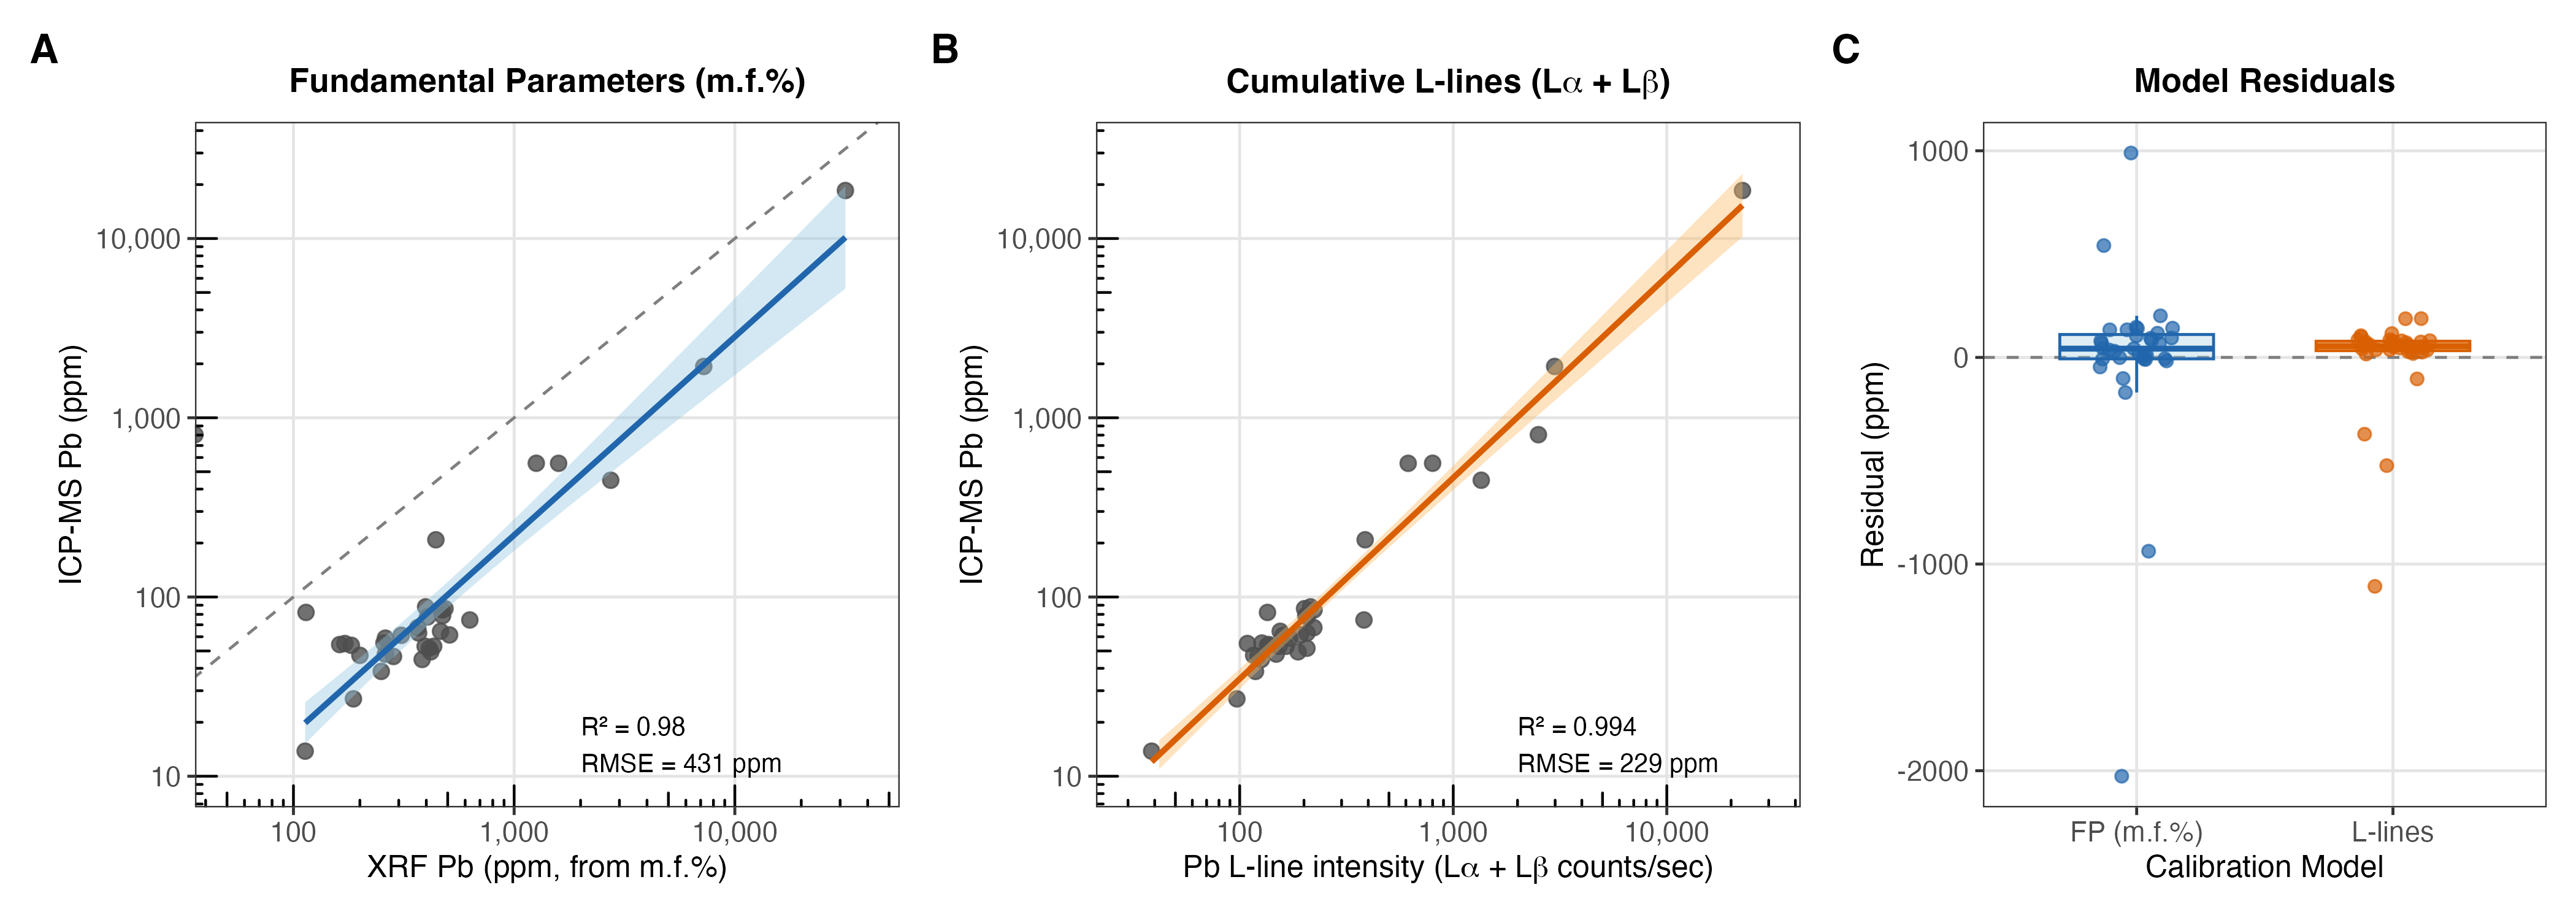
\includegraphics[width=\textwidth]{Fig_XRF_calibration_final.png}
\caption{XRF calibration models for Pb quantification against ICP-MS (n = 35). Log-log scale. (A) Fundamental parameters model using manufacturer-reported wt\%. Dashed line indicates 1:1 relationship. (B) Cumulative L-line intensity model (L$\alpha$ + L$\beta$). (C) Residual distributions for each calibration approach.}
\label{fig:xrf_calibration}
\end{figure}

%------------------------------------------------------------------------------
\subsection{Screening Threshold Classification Performance}

Calibrated XRF models were evaluated for their ability to classify samples as exceeding regulatory screening thresholds of 80, 200, 400, and 1000~ppm Pb (Table~\ref{tab:threshold_classification}, Figure~\ref{fig:threshold_performance}). Based on ICP-MS, 11 (31\%), 7 (20\%), 6 (17\%), and 2 (6\%) of 35 samples exceeded these thresholds, respectively.

Classification performance improved with increasing threshold concentration. At 400 and 1000~ppm, both models achieved equivalent performance: 83\% sensitivity and 100\% specificity at 400~ppm (1 false negative each), and 100\% sensitivity with 97\% specificity at 1000~ppm (1 false positive each).

At lower thresholds, the cumulative L-line model outperformed the FP model. At 200~ppm, the L-line model achieved 86\% sensitivity versus 71\% for FP, with both maintaining 100\% specificity. At 80~ppm, both models achieved 64\% sensitivity, but the L-line model had substantially higher specificity (96\% vs 83\%), producing only 1 false positive compared to 4 for the FP model.

Alternative calibrations excluding high-concentration samples (>400 or >1000~ppm) were evaluated but did not improve overall classification performance. Restricted-range models increased sensitivity at 80~ppm but decreased sensitivity at 400~ppm due to underestimation from shallower regression slopes.

\begin{table}[htbp]
\centering
\caption{Classification performance of calibrated XRF models for Pb screening thresholds (n = 35).}
\label{tab:threshold_classification}
\begin{tabular}{llrrrr}
\toprule
Threshold (ppm) & Model & Sensitivity (\%) & Specificity (\%) & FP & FN \\
\midrule
\multirow{2}{*}{80} & L-lines & 64 & 96 & 1 & 4 \\
 & FP (wt\%) & 64 & 83 & 4 & 4 \\
\midrule
\multirow{2}{*}{200} & L-lines & 86 & 100 & 0 & 1 \\
 & FP (wt\%) & 71 & 100 & 0 & 2 \\
\midrule
\multirow{2}{*}{400} & L-lines & 83 & 100 & 0 & 1 \\
 & FP (wt\%) & 83 & 100 & 0 & 1 \\
\midrule
\multirow{2}{*}{1000} & L-lines & 100 & 97 & 1 & 0 \\
 & FP (wt\%) & 100 & 97 & 1 & 0 \\
\bottomrule
\end{tabular}
\begin{flushleft}
\small{FP = false positives; FN = false negatives. Sensitivity = TP/(TP+FN); Specificity = TN/(TN+FP).}
\end{flushleft}
\end{table}

\begin{figure}[htbp]
\centering
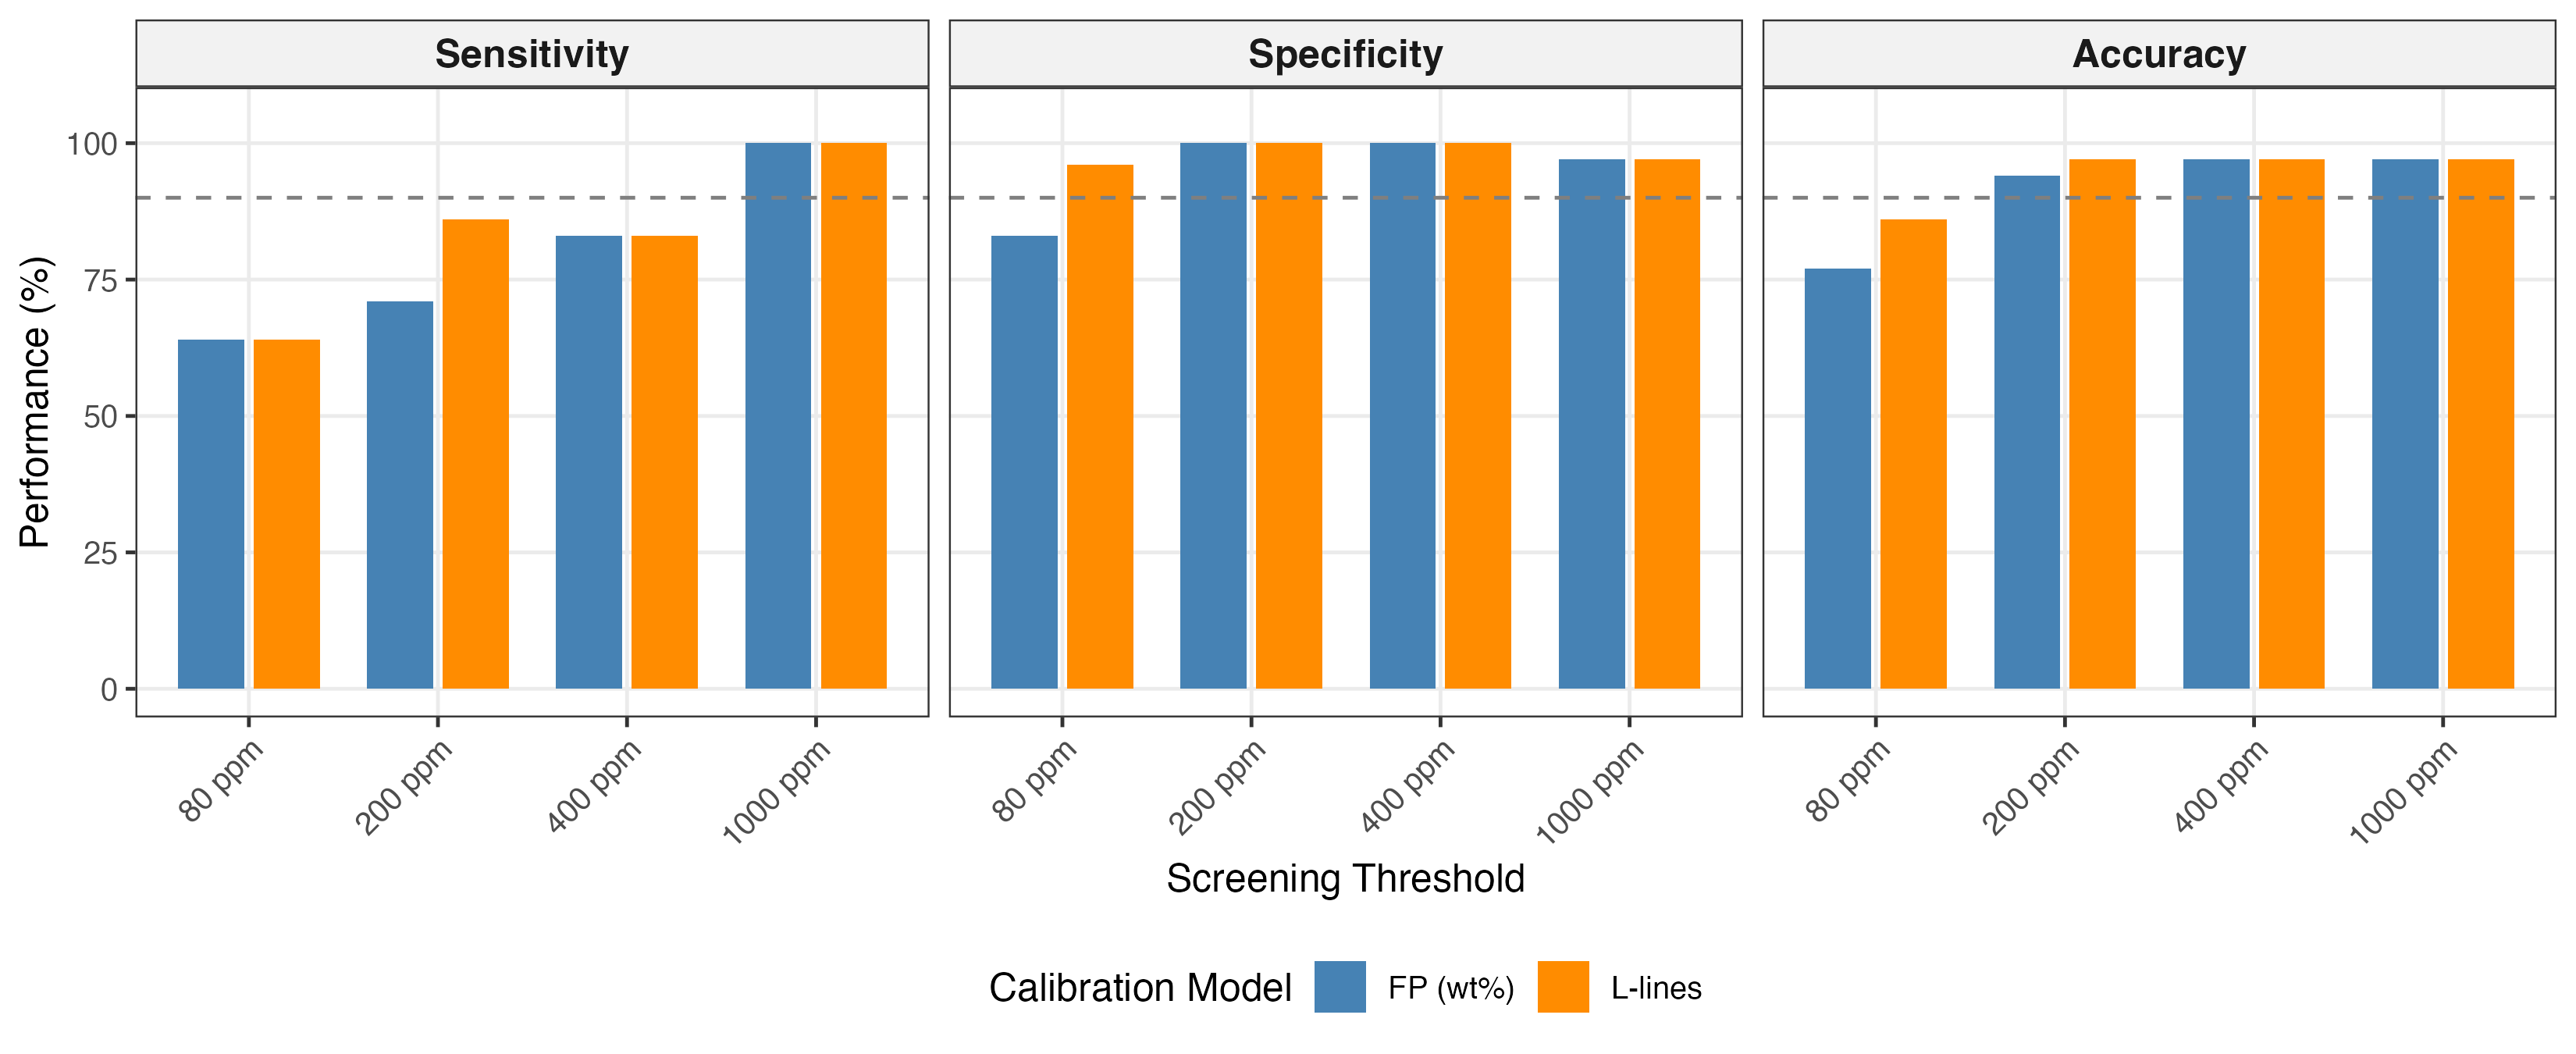
\includegraphics[width=\textwidth]{Fig_threshold_performance_2models.png}
\caption{Classification performance of calibrated XRF models across Pb screening thresholds. Dashed horizontal line indicates 90\% performance benchmark.}
\label{fig:threshold_performance}
\end{figure}

%==============================================================================
\end{document}
